\section{Introduction}

Lepton flavor violation in charged lepton sector (CLFV) such as in 
$\mu^+\to e^+\gamma$ and $\mu^+\to e^+e^-e^+$ is forbidden in
the Standard Model (SM) of particle physics. In neutral lepton sector,
neutrino flavor osicillations have been well established. This could 
mediate charged lepton flavor violation through loop diagrams, but this
process is highly suppressed due to extremely small neutrino masses. 
For example, the branching fraction for
$\mu \to e \gamma$ is~\cite{}
\begin{equation}
BR(\mu \rightarrow e \gamma)=\frac{3\alpha}{32\pi}\left|\sum_i U_{\mu
i}^* U_{e i}\frac{m_{\nu_{i}}^2}{m_{W}^2}\right|^2 \sim 10^{-52},
\end{equation}
where $U_{ei}$ are the leptonic mixing matrix elements, assuming neutrinos
are Dirac particles. This is clearly well below any experiment's reach.
However, in many extensions of the SM such as supersymmetric grand unified
theories or theories with extra dimentions, larger contributions to CLFV are
allowed~\cite{new physics}. Observing CLFV is a clear indication of the 
existence of New Physics. Figure~\ref{CL:mutoegamma} shows sample diagrams
of these processes mediated by SUSY particles.

The effective Lagrangian relevant for the $\mu^+\to e^+\gamma$ and $\mu^+\to e^+e^-e^+$
decays can be parametrized, regardless of the origin of CLFV, as a sum of
the dipole terms and the ``contact terms''; $\mu^+\to e^+\gamma$ is sensitive to
dipole terms only, while both dipole and contact terms contribute to 
$\mu^+\to e^+e^-e^+$~\cite{deGouvea:2013zba}. Pushing the upper limits of
the $\mu^+\to e^+\gamma$ and $\mu^+\to e^+e^-e^+$ branching fractions 
to $10^{-14}$ and $10^{-16}$, respectively, could set the New Physics energy
scale to several thousand TeV level.
An interesting feature of $\mu \rightarrow eee$ is 
the possibility to determine the chirality of New Physics, should it be 
observed with sufficient statistics~\cite{Okada:1999zk}. 

\begin{figure}[htp]
\begin{center}
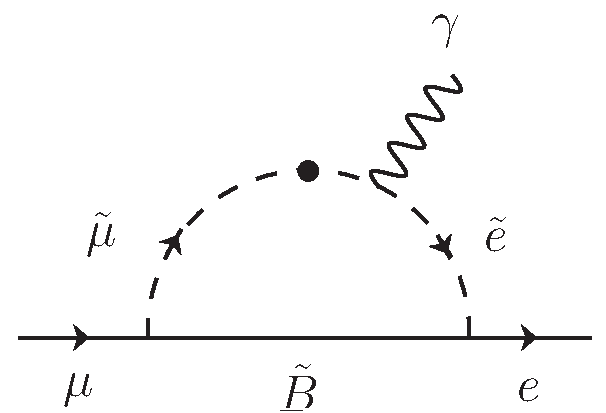
\includegraphics[width=5cm]{Figures/mu_e_gamma_diagram.pdf} \hspace*{2cm}
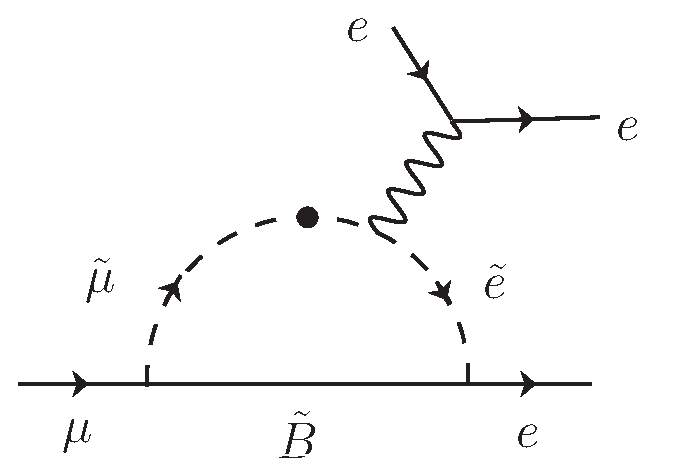
\includegraphics[width=5cm]{Figures/mu_3e_diagram.pdf}
\caption{\label{CL:mutoegamma}$\mu \rightarrow e\gamma$ decay mediated by SUSY particles (left panel), and $\mu \rightarrow 3e$ decay (right panel).}
\end{center}
\end{figure}
